\documentclass[11pt,a4paper]{article}

\usepackage{style2017}
\usepackage{hyperref}

\hypersetup{
    colorlinks =false,
    linkcolor=blue,
   linkbordercolor = 1 0 0
}
\newcounter{numexo}
\setcellgapes{1pt}

\begin{document}



\begin{NSI}
{Exercice}{Processus}
\end{NSI}






\addtocounter{numexo}{1}
\subsection*{\Large Exercice \thenumexo}
\begin{enumerate}
\item Ouvrir le gestionnaire de tâches. Vous pouvez directement saisir la commande \textbf{taskmgr} dans la barre de tâches windows. Assurez-vous d'avoir 
\begin{itemize}
\item tous les détails d'affichage
\item La colonne PID affichée, sinon clic droit sur les entêtes de colonne puis cocher PID.
\end{itemize}


\item Quelles sont les ressources matérielles évaluées par le gestionnaire de tâches (onglet performance) ?
\item Quelle est la fréquence affichée du processeur ?
\item Quel est le nombre de coeurs du processeur ?
\item Quelle est la capacité de la RAM ? Utilisée ? Disponible ?
\item Quelle est la taille du disque dur ?
\item Donner trois caractéristiques du processeur graphique ?
\end{enumerate}


\addtocounter{numexo}{1}
\subsection*{\Large Exercice \thenumexo}
Le bloc-notes peut-il bloquer votre ordinateur ?
\begin{enumerate}
\item Ouvrir le bloc notes et vérifier la présence du processus associé dans le gestionnaire de tâches puis relever :
\begin{enumerate}
\item la quantité de mémoire qui lui est allouée ?
\item le PID de ce processus et son statut.
\end{enumerate}
\item Saisir la phrase "Le bloc notes utilise peu de ressources !" dans le bloc notes.
\begin{enumerate}
\item La quantité de mémoire allouée a-t-elle changé ?
\item Enregistrer votre fichier et contrôler les paramètres du processus. Que remarquez-vous ?
\end{enumerate}
\item Copier votre phrase puis collez-la ? Sélectionnez vos 2 phrases puis collez-les ? Répéter ce copier-coller-enregistrer plusieurs fois.

La quantité de mémoire et de processeur utilisé varie-t-elle ?
\item Le bloc notes peut-il planter l'ordinateur ? Poursuivez vos copier-coller et observer l'évolution du processus ?
\end{enumerate} 



\addtocounter{numexo}{1}
\subsection*{\Large Exercice \thenumexo}
\begin{enumerate}
\item Lancer le navigateur firefox et vérifier la présence du processus dans le gestionnaire de tâches.
\item Combien de processus sont en cours d'exécution ?
\item Est-il possible de mettre fin à des processus sans tous les arrêter ?
\item Un des processus est le parent des autres. Lequel ? Vérifier que tous les autres processus s'arrêtent lorsqu'on met fin au processus parent.
\item Ajouter la colonne "type" et retrouver le processus parent ?
\end{enumerate}



\addtocounter{numexo}{1}
\subsection*{\Large Exercice \thenumexo}
\begin{enumerate}
\item Trier les processus selon leur PID.\begin{enumerate}
\item Quel est le processus qui a la plus petite valeur ?
\item Que signifie la valeur attribuée au processeur ?
\end{enumerate}

\item Lancer le bloc-notes et noter son PID.

\item Dans une console windows, saisir la commande \textbf{tasklist}.
\begin{enumerate}
\item Quel est l'affichage obtenu ?
\item Saisir la commande suivi d'un slash et du point d'interrogation /? . Que renvoie la commande ?
\item Quelle commande faut-il saisir pour afficher le processus associé au bloc-notes ?
\item Lancer firefox puis afficher dans la console la liste des processus associés.
\item Vérifier que le premier de la liste est le parent des autres processus (relancer plusieurs fois firefox).
\item Pour arrêter un processus, on utilise la commande \textbf{taskkill} en indiquant le PID du processus.

Arrêter le bloc-notes et firefox en ligne de commandes.
\end{enumerate}
\end{enumerate}


\addtocounter{numexo}{1}
\subsection*{\Large Exercice \thenumexo}
Cet exercice se réalise sur une machine avec Linux installé.
\begin{enumerate}
\item Ouvrir la console et saisir la commande \textbf{ps -a -u -x}. Que renvoie-t-elle ?
\item Lancer le navigateur web puis vérifier les processus.
\item Pour affiner l'affichage, il est possible d'utiliser la commande \textbf{grep} en complément de la première. On appelle ça un tube ou pipe. 

Voici la syntaxe: \textbf{ps -a -u -x | grep "texte à chercher"}

Afficher uniquement les processus du navigateur web.
\item Il existe une commande qui affiche l'arborescence des processus montrant ainsi la filiation. Cette commande est \textbf{pstree}.
\begin{enumerate}
\item Cette commande est-elle installée sur votre système ? Sinon l'installer.
\item Afficher l'arborescence des processus.
\end{enumerate}
\item La commande \textbf{top} permet de contrôler les processus en temps réel d'exécution.
\begin{enumerate}
\item Afficher les processus actifs.
\item Lancer une application et contrôler sa présence sur la console.
\end{enumerate}
\item La commande qui arrête un processus est \textbf{kill} avec le PID du processus. Arrêter le navigateur web avec cette commande.
\end{enumerate}



\addtocounter{numexo}{1}
\subsection*{\Large Exercice \thenumexo}
\textbf{Cet exercice pourra être réalisé sur Windows et sur Linux.}\bigskip

Python dispose d'un module qui permet d'exécuter des commandes au niveau du système d'exploitation. 

Ce module est \textbf{os}.\medskip

La méthode \textbf{system} de ce module permet d'exécuter une commande. 

Par exemple \textbf{os.system("C:/windows/notepad.exe")} ouvre le bloc notes. On récupère le prompt de l'interpréteur python seulement en fermant l'application ouverte et l'interpréteur affiche alors la valeur 0.\medskip

La méthode \textbf{startfile} permet l'ouverture d'un fichier. 

Elle prend en argument le chemin complet du fichier à ouvrir.\medskip

La méthode \textbf{getpid} renvoie le pid du processus python en cours.

La méthode \textbf{getppid} renvoie le pid du parent du  processus python en cours.\medskip
 
D'autres méthodes utiles sont données ci-après (attention aux arguments):
\begin{itemize}
\item \textbf{name} renvoie le nom de l'OS.
\item \textbf{getcwd} renvoie le répertoire courant.
\item \textbf{listdir} renvoie le contenu du répertoire courant.
\item \textbf{mkdir} crée un répertoire.
\item \textbf{chdir} change de répertoire courant
\item \textbf{remove} supprime un fichier.
\item \textbf{rmdir} supprime un répertoire.
\item \textbf{name} renvoie le nom de l'OS.
\end{itemize}

Ouvrir l'interpréteur python et importer le module \textbf{os}. 
Toutes les actions demandées ci-après se font \textbf{exclusivement} en python.\medskip

\begin{enumerate}
\item Afficher le nom du système d'exploitation.
\item Quel est le répertoire courant ?
\item Lister le contenu du répertoire courant. 
\begin{enumerate}
\item Combien y a-t-il de dossiers et fichiers dans le répertoire courant ?
\item Un fichier et un dossier sont cachés si le nom commence par un point. Pouvez-vous trouver combien il y en a ?
\end{enumerate}
\item Créer un répertoire \textbf{titi} dans le répertoire courant puyis placez-vous dans le répertoire \textbf{titi}.
\item Afficher le PID du processus python en cours d'utilisation. Celui du parent aussi.
\item Ouvrir le gestionnaire de tâches. Vérifier les PID de python et de son parent.
\item Arrêter le processus python en cours d'exécution avec une commande python.
\end{enumerate}

-
\addtocounter{numexo}{1}
\subsection*{\Large Exercice \thenumexo}
Il existe une autre manière de procéder avec le module \textbf{subprocess}.

\begin{enumerate}
\item Dans un environnement windows, saisir les commandes suivantes et relever ce qui se passe:
\begin{flushleft}
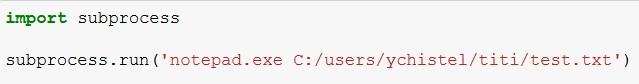
\includegraphics[scale=0.8]{img/subprocess1.jpg}
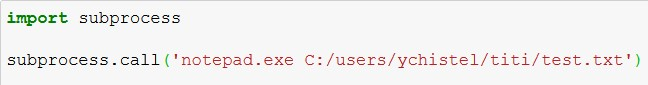
\includegraphics[scale=0.8]{img/subprocess2.jpg}
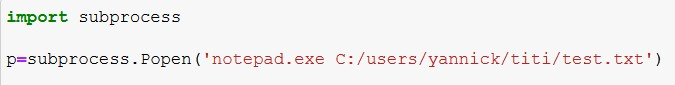
\includegraphics[scale=0.8]{img/subprocess3.jpg}
\end{flushleft}
\item Quelle méthode semble la plus intéressante ? Pourquoi?
\item On utilise la troisième méthode et notre objet p qui est un processus en cours d'exécution. 
\begin{enumerate}
\item Quelle méthode renvoie le pid du processus en cours ?
\item Quelle méthode permet d'arrêter le processus en cours ?
\end{enumerate}
\item Écrire un script python:
\begin{enumerate}
\item Qui permet d'exécuter un navigateur comme Firefox ou Chrome en affichant la page d'accueil du site du lycée.
\item Affiche le PID du processus du navigateur 
\item Termine le processus.
\end{enumerate}
\item Tester ce module dans un environnement linux.
\end{enumerate}


\addtocounter{numexo}{1}
\subsection*{\Large Exercice \thenumexo}
On considère trois processus $P_1$, $P_2$ et $P_3$ et trois ressources $R_1$, $R_2$ et $R_3$ qui s'exécutent les uns après les autres selon :
\begin{itemize}
\item[$P_1$]: demande $R_1$, demande $R_2$, libère $R_1$, libère $R_2$.
\item[$P_2$]: demande $R_2$, demande $R_3$, libère $R_2$, libère $R_3$.
\item[$P_3$]: demande $R_3$, demande $R_1$, libère $R_3$, libère $R_1$.
\end{itemize}
\begin{enumerate}
\item Y a-t-il interblocage ?
\item Décrire une exécution de trois processus qui conduit à une situation d'interblocage.
\item Représenter cette situation par un schéma.
\end{enumerate}


%\addtocounter{numexo}{1}
%\subsection*{\Large Exercice \thenumexo}
%Le Raspberry Pi (RPI), modèle 4, est un nano-ordinateur dont la taille nécessite qu'il soit équipé d'un SOC.\medskip
%
%La carte mère du RPI, document 2, contient différents composants pour 
%
%\textbf{Document 1}\hspace{6.2cm}\textbf{Document 2}\medskip
%
%\includegraphics[scale=0.5]{img/rpi4b.jpg}
%\includegraphics[scale=0.4]{img/ARM-processeur-Cortex-A72.jpg}
%
%En utilisant les documents ci-dessus, répondre aux questions suivantes:\medskip
%
%\begin{enumerate}
%\item Qu'est-ce qu'un SoC ?
%\item Donner la désignation du SoC du raspberry pi modèle 4.
%\item Donner les caractéristiques du processeur du RPI.
%\item Quelle(s) quantité(s) de mémoire possède un RPI ?
%\item Donner 5 entrées/sorties disponibles sur le RPI.
%\end{enumerate}
%
%\addtocounter{numexo}{1}
%\subsection*{\Large Exercice \thenumexo}
%Cet exercice nécessite l'utilisation d'une carte raspberry pi.
%
%\begin{enumerate}
%\item Ouvrir un terminal et entrer la commande \textbf{pinout}. Quel est le nom du Soc et la quantité de RAM disponible ?
%\item Entrer la commande \textbf{cat /proc/cpuinfo}. Noter les trois dernières lignes correspondant au type de hardware, au code de révision et au numéro de série.
%\item Le numéro de révision est noté en hexadécimal. Convertir cette écriture en binaire (24 bits).
%\item Le numéro de révision regroupe des informations en regroupant les bits de gauche à droite:
%$b_1b_2b_3......b_{23}b_{24}$.
%\begin{enumerate}
%\item La valeur de $k=b_2b_3b_4$ donne la taille de la mémoire : $2^{8+k}$ Mo. Est-ce conforme ?
%\item La valeur $b_5b_6b_7b_8$ correspond au fabricant : 0 pour Sony UK, 1 pour Egoman, 2 pour Embest, 3 pour Sony Japan, 4 pour Embest, 5 pour Stadium.
%\item La valeur des 4 bits suivants, de $b_9$ à $b_{12}$ correspond au processeur. Quelle est la valeur de notre processeur ?
%\item Les huit bits suivants nous donne le modèle du RPI. En utilisant le tableau ci-dessous, identifier ce modèle.
%
%\begin{tabular}{|L{2.5cm}*{6}{|C{1.5cm}}|}\hline
%numéro & 0 & 1 & 2 & 3 & 4 & 5\\\hline
%modèle & A & B & A+ & B+ & 2B & Alpha\\\hline
%numéro & 6 & 7 & 8 & 9 & 10 & 11\\\hline
%modèle & CM1 & & 3B & Zero & CM3 & Zero W\\\hline
%numéro & 12 & 13 & 14 & 15 & 16 & 17\\\hline
%modèle &  & 3B+ & 3A+ & & CM3+ & 4B\\\hline
%\end{tabular}\medskip
%
%\item Les quatre derniers bits donnent le numéro de révision. Quel est ce numéro de révision ?
%
%Vérifier avec la commande \textbf{cat /sys/firmware/devicetree/base/model}.
%\end{enumerate}
%
%\end{enumerate}


\end{document}
